\documentclass[final]{beamer}

\usepackage[size=custom,width=16,height=9,scale=0.50]{beamerposter}
\usepackage[utf8]{inputenc}
\usepackage{graphicx}
\usepackage{tikz}
\usepackage{xcolor}
\usepackage{booktabs}
\usepackage{enumitem}

% Colors
\definecolor{washured}{RGB}{163,0,52}
\definecolor{lightgray}{RGB}{251,251,251}

% Global style
\setbeamertemplate{navigation symbols}{}
\setbeamersize{text margin left=0cm, text margin right=0cm}
\setbeamertemplate{blocks}[rounded][shadow=false]
\setbeamercolor{block title}{fg=white,bg=washured}
\setbeamercolor{block body}{fg=black,bg=lightgray}

% Block title and spacing
\setbeamerfont{block title}{size=\fontsize{5}{6}\selectfont,series=\bfseries}
\addtobeamertemplate{block begin}{\vspace{0.2ex}}{}
\addtobeamertemplate{block end}{}{\vspace{0.6ex}}

\begin{document}

\begin{frame}[t,fragile]

% =========================
% Top title bar (flush to top)
% =========================
\noindent
\colorbox{washured}{%
    \parbox[c][0.23in][c]{\paperwidth}{%
        \hspace*{0.10cm}%
        {\color{white}\fontsize{10}{11}\selectfont\bfseries
        Customer Churn Prediction \& Retention Analysis}%
    }%
}

\vspace{0.01in}

% =========================
% Three-column layout
% Wider columns, safe spacing, fully visible right column
% =========================
\noindent
\makebox[\paperwidth][c]{%
\begin{minipage}{0.98\paperwidth}
\begin{columns}[t,totalwidth=0.98\paperwidth]

% ---------- Left column ----------
\begin{column}{0.305\paperwidth}

    \begin{block}{1. Executive Summary}
    \fontsize{4.8}{5.6}\selectfont

    \textbf{Core Objective}\\
    Define target (Churn) and remove leakage variables. Drop identifiers and redundant features (e.g., Total Charges, CLTV). CLTV validated via correlation with existing variables.

    \vspace{0.04in}

    \textbf{Preprocessing:}\\
    • Numerical: median imputation + standardization\\
    • Categorical: mode imputation + one-hot encoding
    \end{block}

    \begin{block}{2. Data Processing}
    \centering

    \begin{minipage}{0.48\linewidth}
        \centering
        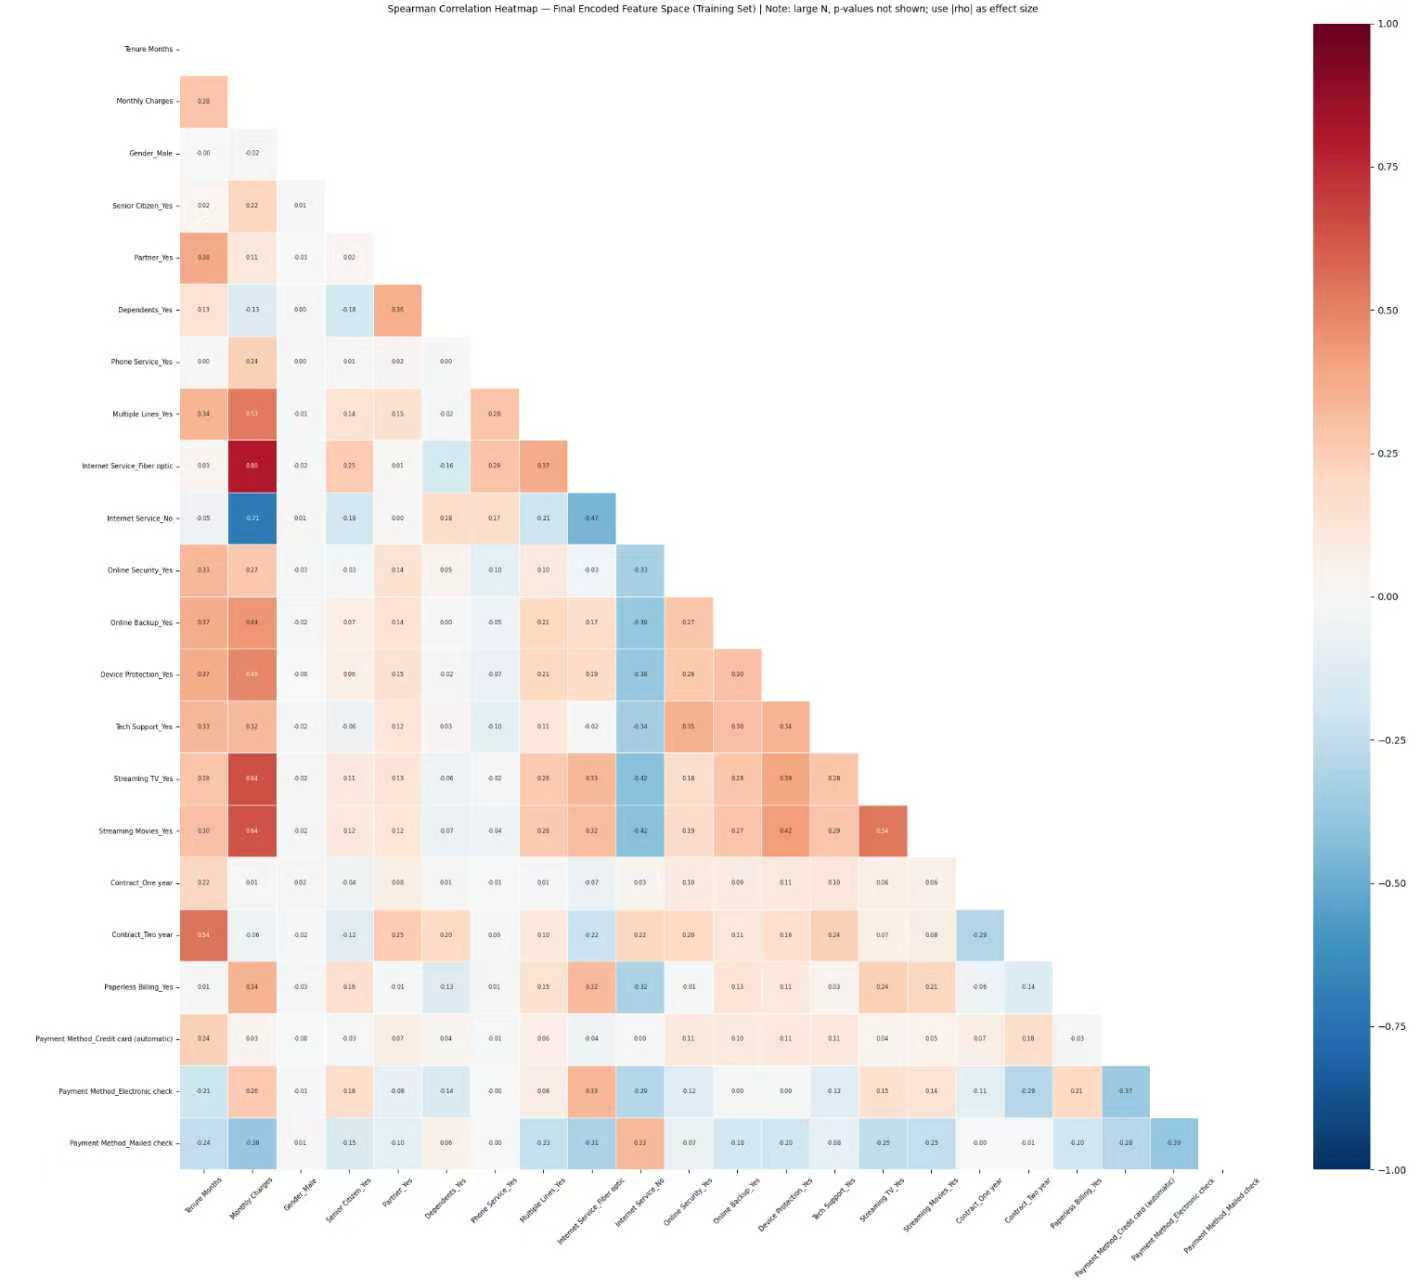
\includegraphics[width=\linewidth]{heatmap.jpg}
        \vspace{-0.8cm}

        {\fontsize{4}{4.8}\selectfont (a) Correlation Heatmap}
    \end{minipage}
    \hfill
    \begin{minipage}{0.48\linewidth}
        \centering
        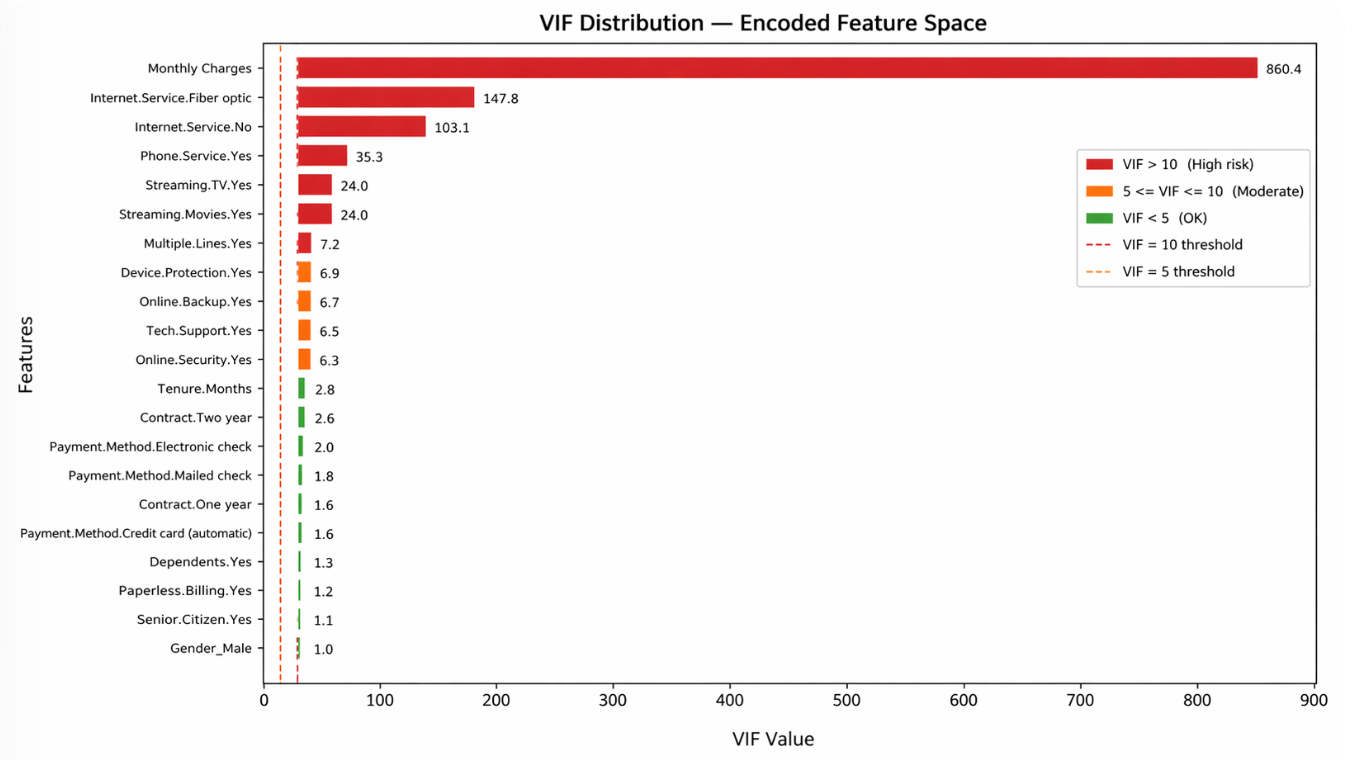
\includegraphics[width=\linewidth]{VIF.png}
        \vspace{-0.35cm}

        {\fontsize{4}{4.8}\selectfont (b) VIF}
    \end{minipage}

    \par\vspace{0.03cm}

    \begin{minipage}{\linewidth}
    \raggedright
    \fontsize{4.8}{5.4}\selectfont
    Low--moderate correlations indicate weak direct relationships.
    VIF reveals multicollinearity from one-hot encoding and overlapping features.
    \end{minipage}

    \par\vspace{0.04cm}

    \centering
    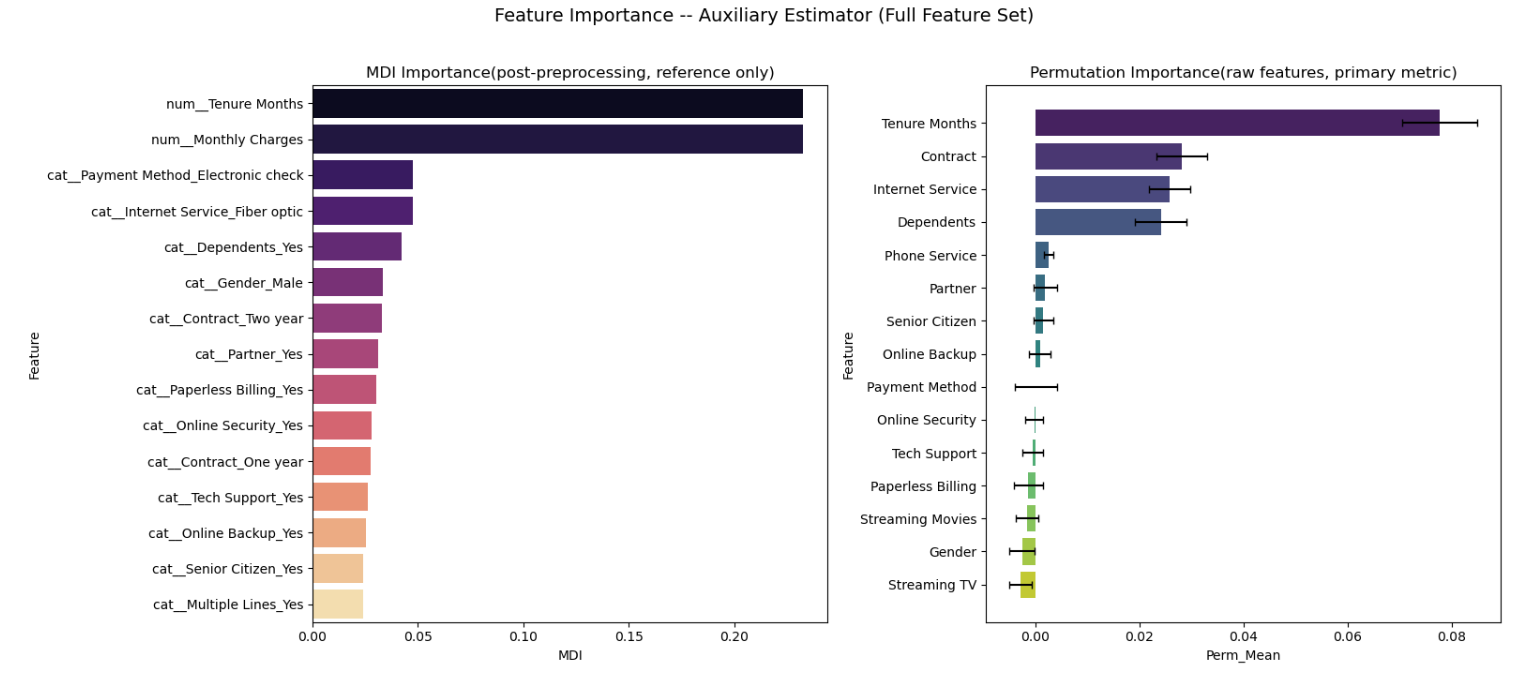
\includegraphics[width=\linewidth]{feature.png}

    \par\vspace{0.02cm}

    \begin{minipage}{\linewidth}
    \raggedright
    \fontsize{4.8}{5.4}\selectfont
    MDI is biased toward numerical and high-cardinality features.
    We rely on permutation importance for more reliable estimates.

    \vspace{0.03cm}

    Two strategies:\\
    Full (18 features): maximize performance\\
    Reduced (4 features): improve interpretability and reduce multicollinearity
    \end{minipage}
    \end{block}

\end{column}

\hspace{0.012\paperwidth}

% ---------- Middle column ----------
\begin{column}{0.305\paperwidth}

    \begin{block}{3. Model Performance}
    \fontsize{4.8}{5.6}\selectfont
    \centering

    % 3.1 Logistic Regression
    \textbf{3.1 Logistic Regression}\\

    \begin{minipage}{0.32\linewidth}
        \centering
        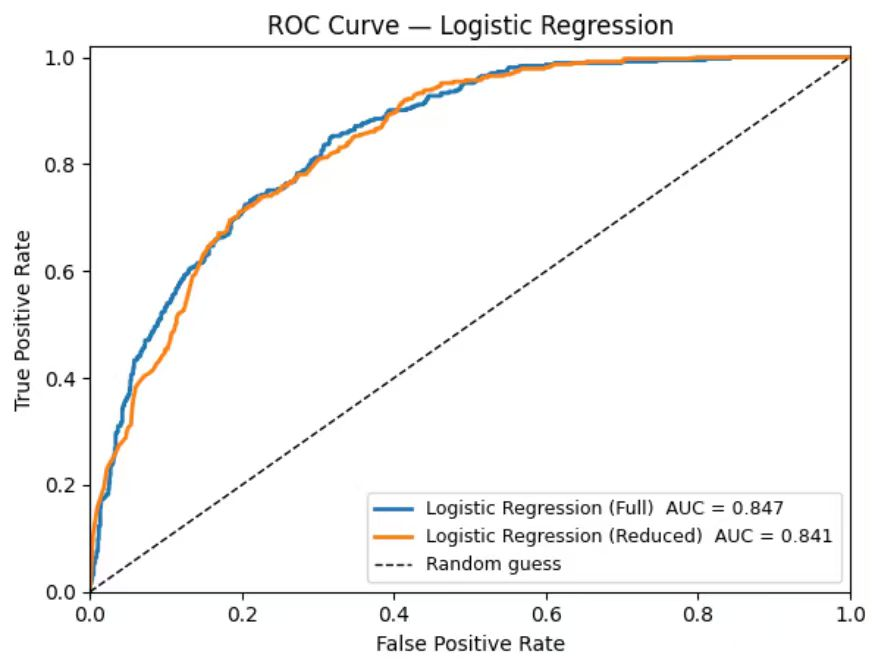
\includegraphics[width=\linewidth]{logis.jpg}
        \vspace{-0.15cm}

        {\fontsize{4}{4.8}\selectfont (a) ROC Curve}
    \end{minipage}
    \hfill
    \begin{minipage}{0.32\linewidth}
        \centering
        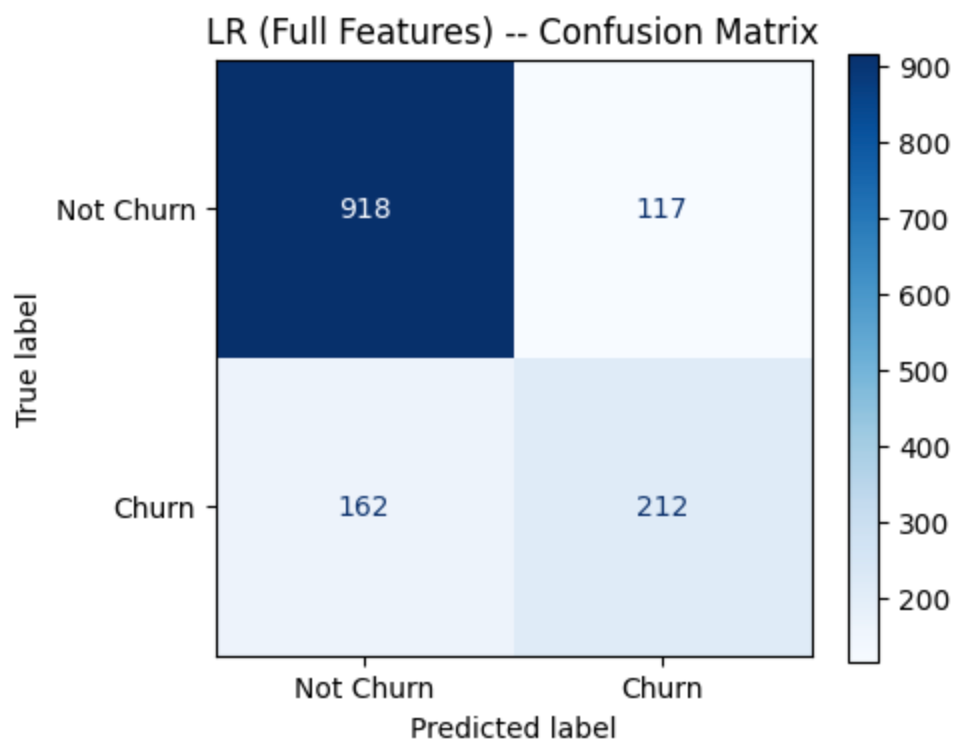
\includegraphics[width=\linewidth]{LRF.png}
        \vspace{-0.15cm}

        {\fontsize{4}{4.8}\selectfont (b) Full Features}
    \end{minipage}
    \hfill
    \begin{minipage}{0.32\linewidth}
        \centering
        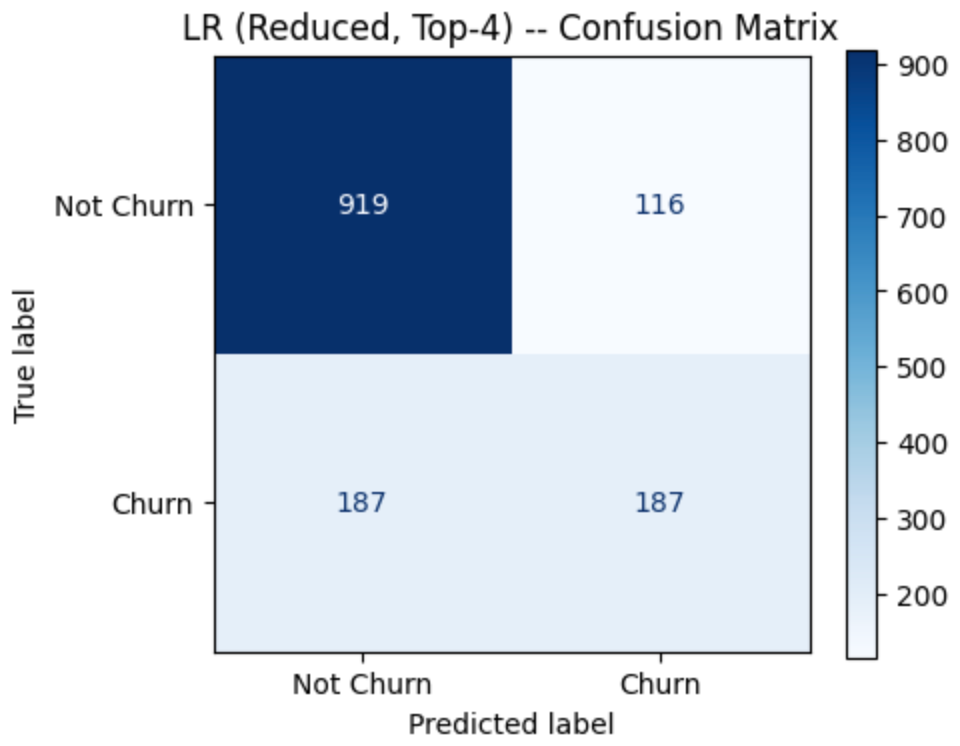
\includegraphics[width=\linewidth]{LR4.png}
        \vspace{-0.15cm}

        {\fontsize{4}{4.8}\selectfont (c) 4 Features}
    \end{minipage}

    \par\vspace{0.05cm}

    \begin{minipage}{\linewidth}
    \raggedright
    \fontsize{4.6}{5.2}\selectfont
    The ROC curves show that the full model achieves a slightly higher AUC (0.847 vs 0.841), indicating better discrimination ability. The confusion matrices also suggest that the full model identifies more churn cases, while the reduced model misses more positives.
    \end{minipage}

    \par\vspace{0.06cm}

    % 3.2 Random Forest
    \textbf{3.2 Random Forest}\\

    \begin{minipage}{0.32\linewidth}
        \centering
        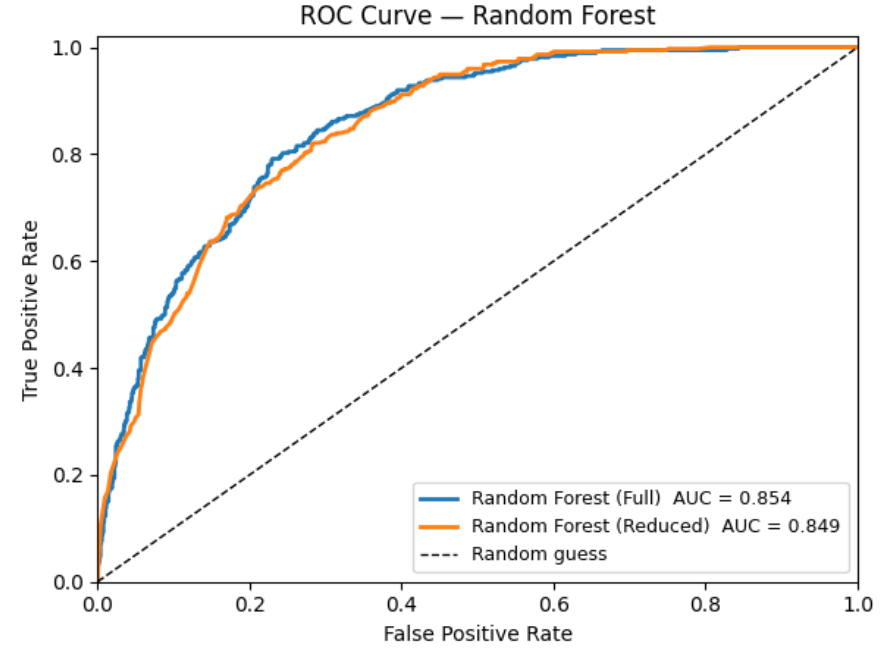
\includegraphics[width=\linewidth]{RandF.png}
        \vspace{-0.15cm}

        {\fontsize{4}{4.8}\selectfont (a) ROC Curve}
    \end{minipage}
    \hfill
    \begin{minipage}{0.32\linewidth}
        \centering
        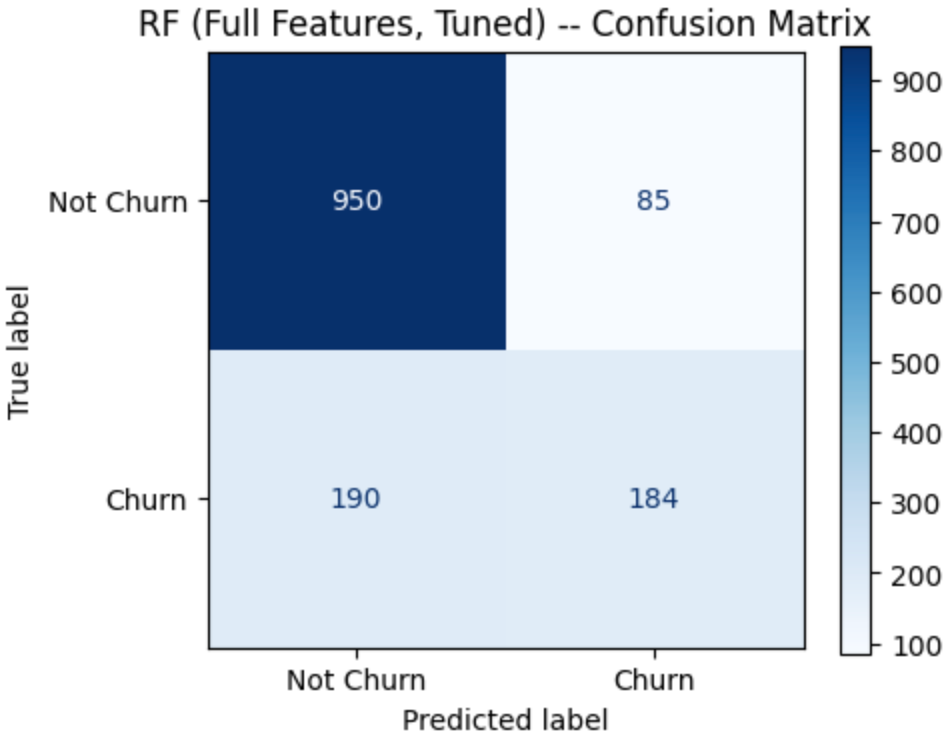
\includegraphics[width=\linewidth]{RFF.png}
        \vspace{-0.15cm}

        {\fontsize{4}{4.8}\selectfont (b) Full Features}
    \end{minipage}
    \hfill
    \begin{minipage}{0.32\linewidth}
        \centering
        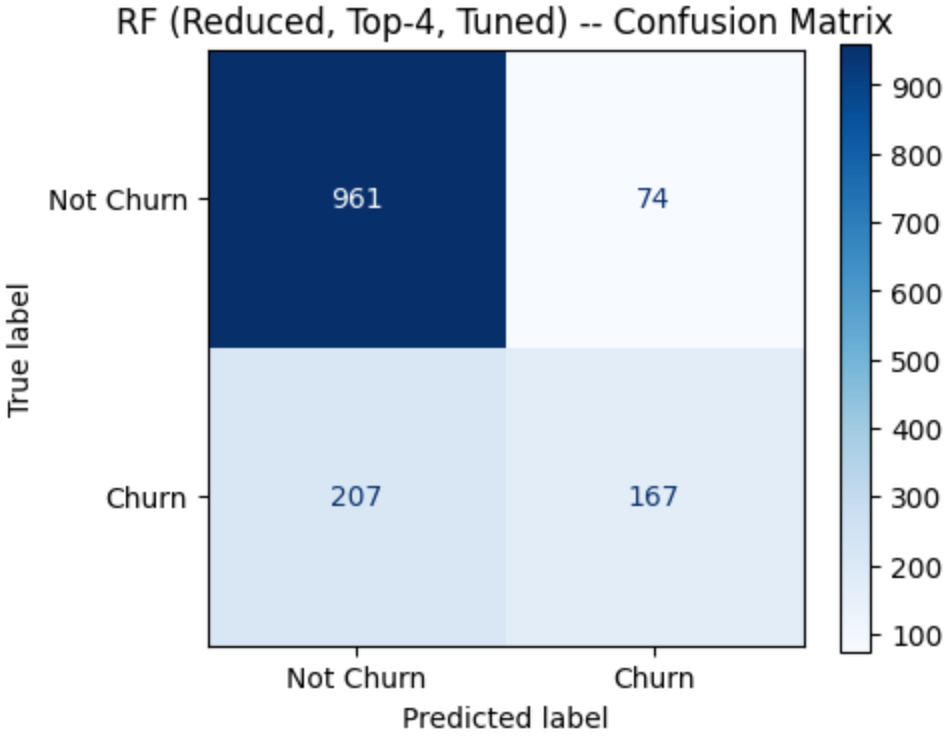
\includegraphics[width=\linewidth]{RF4.png}
        \vspace{-0.15cm}

        {\fontsize{4}{4.8}\selectfont (c) 4 Features}
    \end{minipage}

    \par\vspace{0.05cm}

    \begin{minipage}{\linewidth}
    \raggedright
    \fontsize{4.6}{5.2}\selectfont
    Full model: Acc 0.805, Rec 0.492, F1 0.572, AUC 0.854\\
    Reduced model: Acc 0.801, Rec 0.447, F1 0.543, AUC 0.849\\
    Full model detects more churn (184 vs 167), with fewer misses.
    \end{minipage}

    \par\vspace{0.06cm}

    % 3.3 XGBoost
    \textbf{3.3 XGBoost}\\

    \begin{minipage}{0.32\linewidth}
        \centering
        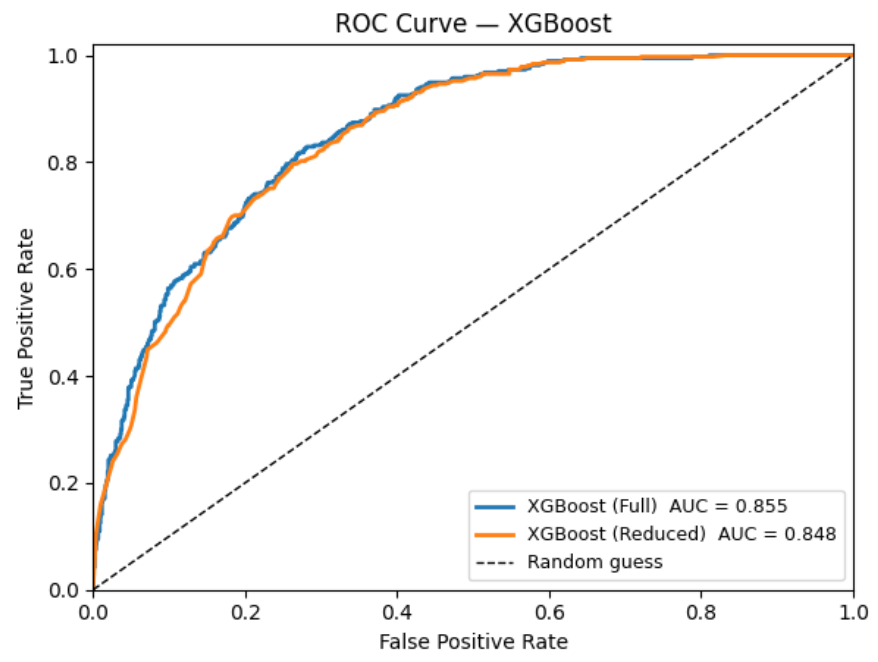
\includegraphics[width=\linewidth]{XG.png}
        \vspace{-0.15cm}

        {\fontsize{4}{4.8}\selectfont (a) ROC Curve}
    \end{minipage}
    \hfill
    \begin{minipage}{0.32\linewidth}
        \centering
        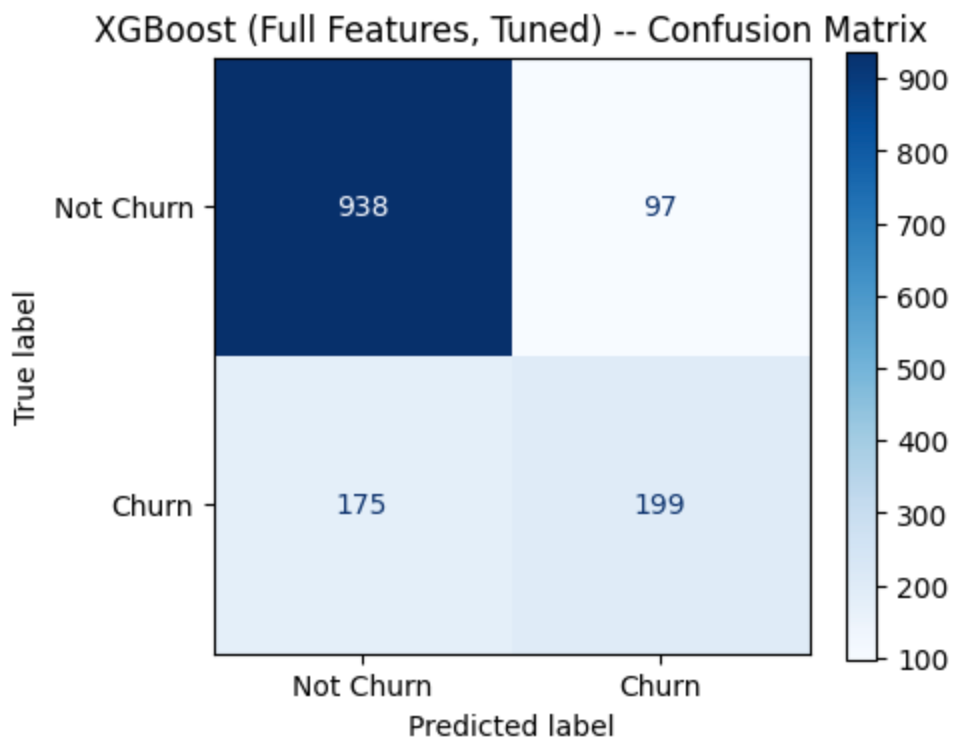
\includegraphics[width=\linewidth]{XGF.png}
        \vspace{-0.15cm}

        {\fontsize{4}{4.8}\selectfont (b) Full Features}
    \end{minipage}
    \hfill
    \begin{minipage}{0.32\linewidth}
        \centering
        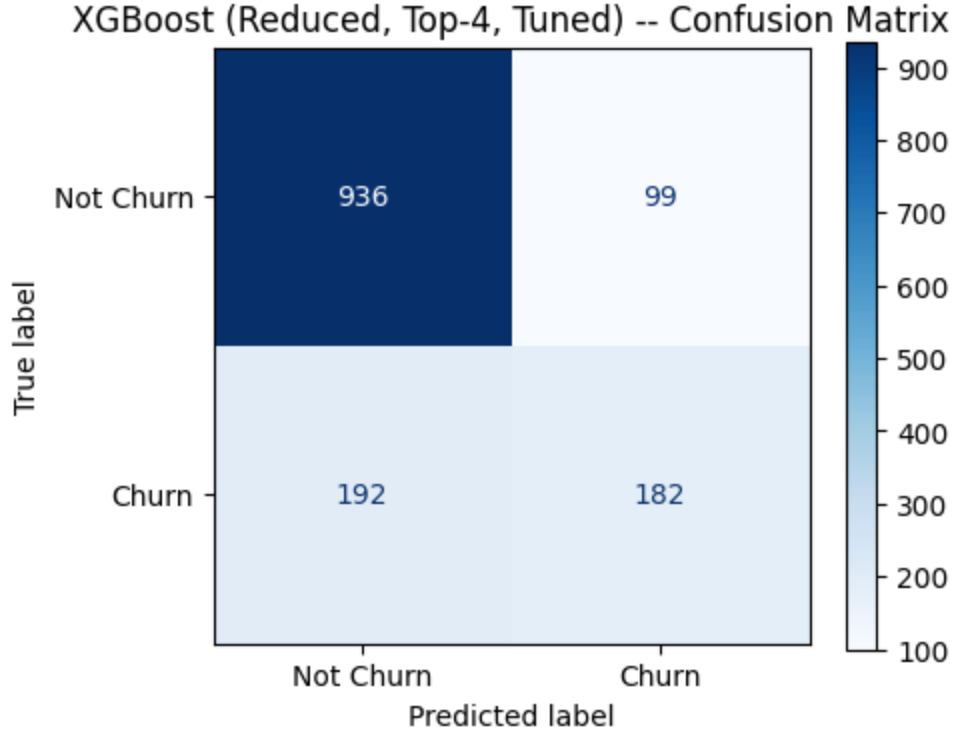
\includegraphics[width=\linewidth]{XG4.png}
        \vspace{-0.15cm}

        {\fontsize{4}{4.8}\selectfont (c) 4 Features}
    \end{minipage}

    \par\vspace{0.05cm}

    \begin{minipage}{\linewidth}
    \raggedright
    \fontsize{4.6}{5.2}\selectfont
    Using the optimized parameters, we train two models on different feature sets. With the full feature set, the model achieves ROC-AUC of 0.855. With the reduced feature set, performance slightly decreases, with ROC-AUC of 0.848.
    \end{minipage}

    \end{block}

\end{column}

\hspace{0.012\paperwidth}

% ---------- Right column ----------
\begin{column}{0.305\paperwidth}

    \begin{block}{4. Final Conclusion}
    \centering

    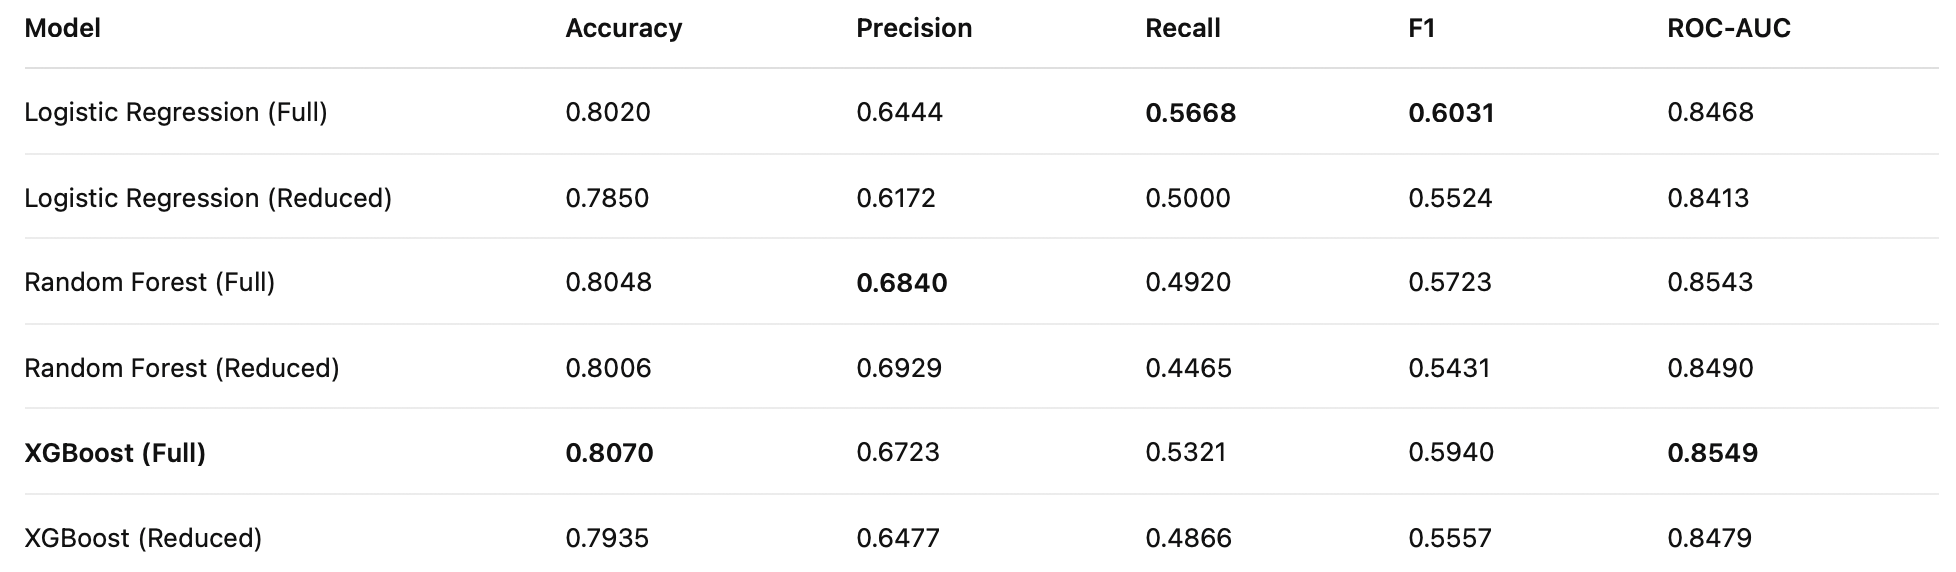
\includegraphics[width=\linewidth]{Conc.png}

    \par\vspace{0.03cm}

    \begin{minipage}{\linewidth}
    \raggedright
    \fontsize{4.6}{5.2}\selectfont
    Among all six experiments, XGBoost with the full feature set achieves the highest ROC-AUC (0.8549), indicating the best overall discriminative ability.

    \vspace{0.03cm}

    Compared with Logistic Regression and Random Forest, XGBoost consistently delivers stronger performance, especially in capturing non-linear relationships and improving recall for churn customers.

    \vspace{0.03cm}

    Additionally, the full feature set is preferred, as it preserves all available information and allows the model to leverage complex interactions among variables, which is critical for accurately predicting customer churn.

    \vspace{0.03cm}

    Therefore, XGBoost (Full Features) is selected as the final model, as it provides the best balance of predictive performance and comprehensive feature utilization.
    \end{minipage}

    \end{block}

\end{column}

\end{columns}
\end{minipage}%
}
\end{frame}
\end{document}